\documentclass[11pt,letterpaper]{article}
\usepackage{amsmath, amssymb, amsbsy}
\usepackage{cite, graphicx}
\usepackage{geometry}
\usepackage{subcaption}

\usepackage[usenames,dvipsnames]{xcolor} 

\usepackage[utf8]{inputenc}

\geometry{letterpaper,nohead,margin=1.4in}
\parindent1em
\parskip0pc
\linespread{1.0}
\pagestyle{plain}

\newcommand{\com}[1]{\hspace{2em}\textrm{#1}} % comments
\newcommand{\sinc}[0]{\textrm{sinc}}
\newcommand{\sign}[0]{\textrm{sign}}
\newcommand{\vv}[1]{\mathbf{#1}} % vector
\newcommand{\p}[0]{\mathbb{P}}
\newcommand{\e}[0]{\mathbb{E}}
\newcommand{\var}[0]{\textrm{Var}}

\title{Learning From Data Problems: Chapter I}
\date{}
\author{J. David Giese}

\begin{document}
\maketitle

\section*{Exercise 1.4}
See \texttt{exercise1_4.py} for code.  Usually the algorithm takes 20 - 40 iterations to run, and matches the result fairly well.  Of course, it depends on the training dataset.

\section*{Exercise 1.5}
a) Learning \\
b) Design \\
c) Learning \\
d) Design \\
e) Design - I am not certain.  The road system is interconnected, so gathering enough data for all the possible situations may be unfeasible.  A simulation with parameters extracted from data may be more useful. \\

\section*{Exercise 1.6}
a) Reinforcement learning, or supervised learning.  In this example, what is the input space and output space?  What training samples do we have?  Assuming the input space is the set of all books, and the output space is whether a \emph{particular person} will buy that book (i.e. ${\textrm{buy}, \textrm{don't buy}}$), then one may view this as supervised learning.  However, just knowing the title of the book is probably not enough information.

A more useful input space would contain details about a particular person's book preferences and even their current mood, and the output space would be, for example, 5 books we should recommend.  Unlike our first approach, this target function can be used on more than one person.  In this case, our training data is likely of the form:

\begin{equation*}
    (\textrm{individual's buying history and mood}, \textrm{suggested book}, \textrm{buy})
\end{equation*}

Thus, this is clearly a reinforcement learning problem.
\\\\
b) Reinforcement learning.  The input space would be a particular tic-tack-toe situation (i.e. for each of the 9 squares, whether it was "x", "o", or "blank").  The output space would be which move should be chosen by the current player.  We would reinforce moves that ultimately led to the person winning the game.
\\\\
c) This could be supervised learning OR unsupervised learning, depending on the training samples we had available.  As supervised learning, the output space would be the set of all movie categories, and our training samples would have the movie (or its mathematically reduced description) as the input value and the category as the output value.  As unsupervised learning, we would only know the movie (or its mathematically reduced description).
\\\\
d) Reinforcement learning.  The input space would, perhaps, be a melody and some parameters describing the style of music desired.  The output would be the produced music.  We would reinforce on how ``good'' listeners thought think the music is.
\\\\
e) Reinforcement learning.  The input space is details about the persons financial history.  The output space is the maximum credit.  We would reinforce on how much money the bank made (or lost) on the person.

\section*{Problem 1.1}
\begin{align*}
    \p(\textrm{2nd B}) &=
    \p(\textrm{BB Bag}) \cdot \p(\textrm{2nd B}|\textrm{BB Bag}) + \p(\textrm{BW Bag}) \cdot \p(\textrm{2nd B}|\textrm{BW Bag}) \\
    &= \frac{1}{2}\cdot 1 + \frac{1}{2} \cdot 0 = \frac{1}{2}
\end{align*}

\section*{Problem 1.2}
a) The $+1$ and $-1$ regions are separated by the line where 
\begin{equation*}
    \vv{w}^T\vv{x} = w_0 + w_1 x_1 + w_2 x_2 = 0
\end{equation*}
this can be rearranged so that
\begin{equation*}
    x_2 = -\frac{w_0}{w_2} - \frac{w_1}{w_2}x_1
\end{equation*}
thus we see $a = -\frac{w_0}{w_2}$ and $b = -\frac{w_1}{w_2}$.  The last important detail is which side is the $+1$ region and which is the $-1$ region.  The $x$-intercept of the dividing line makes a good reference point.  By looking at a point just to the right of the $x$-intercept, $x_+ = (1, -\frac{w_0}{w_1} + \delta, 0)$ we see $h(\vv{x_+}) = \sign(\vv{w}^T \vv{x_+}) = \sign(\delta \cdot w_1)$.  Thus if $w_1 > 0$ the $+$ region is the right, and vice versa. \\\\
b) The two cases are identical, except that the $+$ region is to the right for the first one, and to the left for the second.  \\\\
Note that the there is a free ``magnitude'' inherent in $\vv{w}$.  Two numbers are required to specify the dividing line, and a ``sign'' is required to indicate which side is the positive side and which is the negative, thus there is a free ``magnitude'' left from the third number.  For example $\vv{w} = (-1, 1, 0)$ is equivalent to $\vv{w} = (-2, 2, 0)$, but not equivalent to $\vv{w} = (1, -1, 0)$.  Interpreting problem 1.3 would be easier if a constraint where placed on $\vv{w}$ to ensure a canonical form.  I propose requiring $w_1^2 + ... + w_d^2 = 1$, which would make $w_0$ a proper threshold, and the remaining portion of $\vv{w}$ a unit vector.  This canonical form simplifies the interpretation of the limits in problem 3 properly.

\section*{Problem 1.3}

a) Since $\vv{w}^*$ separates the data, we know $h(\vv{x}) = \sign(\vv{w}^{*T}\vv{x}_n) = y_n \; \forall n$, thus we have

\begin{equation*}
    y_n(\vv{w}^{*T}\vv{x}_n) = y_n(\sign(\vv{w}^{*T}\vv{x}_n)|\vv{w}^{*T}\vv{x}_n|) = y_n^2 |\vv{w}^{*T}\vv{x}| = |\vv{w}^{*T}\vv{x}_n| \ge 0
\end{equation*}
thus we have $\rho \ge 0$.  If one further assumes that no data points fall on the dividing line, we have $\rho > 0$.
\\\\
b) I'm not sure why they need the first equation here, as it isn't necessary to prove the second part of the problem, but for thoroughness we have from (a)

\begin{align*}
     y(t)(\vv{x}^T(t)\vv{w}^*) &\ge \min y(t)(\vv{w}^{*T}\vv{x}(t)) > \rho \; \forall t \quad \Longrightarrow \\
     y(t - 1)(\vv{x}^T(t - 1)\vv{w}^*) &> \rho \quad \Longrightarrow \\
     \vv{w}^T(t - 1)\vv{w}^*  + y(t - 1)(\vv{x}^T(t - 1)\vv{w}^*) &> \vv{w}^T(t - 1)\vv{w}^* + \rho \quad \Longrightarrow \\
     (\vv{w}^T(t - 1) + y(t - 1)\vv{x}(t - 1))\vv{w}^* &> \vv{w}^T(t - 1)\vv{w}^* + \rho \quad \Longrightarrow \\
     \vv{w}^T(t)\vv{w}^* &> \vv{w}^T(t - 1)\vv{w}^* + \rho.
\end{align*}
Now for the interesting part: let $S(t)$ be the claim that $\vv{w}^T\vv{w}^* \ge t\rho$.  We know $S(0)$ is true because $\vv{w}(0) = \vv{0}$.  We assume $S(t)$, and have

\begin{align*}
 \vv{w}^T(t)\vv{w}^* &> t\rho \quad \Longrightarrow \\
 (\vv{w}^T(t) + y(t)\vv{x}^T(t))\vv{w}^* &> t\rho +  y(t)\vv{x}^T(t)\vv{w}^* \quad \Longrightarrow \\
 \vv{w}^T(t + 1)\vv{w}^* &> t\rho +  y(t)\vv{x}^T(t)\vv{w}^* \quad \Longrightarrow \\
 \vv{w}^T(t + 1)\vv{w}^* &> (t + 1)\rho,
\end{align*}
Thus by induction we have $S(t)$ to be true for all $t$.
\\\\
Note that it would seem $\vv{w}$ diverges, however eventually you will run out of bad data points if the data is linearly separable.
\\\\
c) Using the fact that $y(t-1)\vv{w}^T(t - 1)\vv{x}(t-1) < 0$ because $y(t-1)$ and $\vv{w}^T(t-1){x}(t-1)$ have opposite signs, we have

\begin{align*}
    ||\vv{w}(t)||^2 &= ||\vv{w}(t - 1)||^2 + y(t-1)^2||\vv{x}(t - 1)||^2 + 2 y(t-1)\vv{w}^T(t - 1)\vv{x}(t-1) \\
    &< ||\vv{w}(t - 1)||^2 + ||\vv{x}(t-1)||^2.
\end{align*}

d) Let $S(t)$ be the claim that $||\vv{w}||^2 \le tR^2$.  We know $S(0)$ is true because $\vv{w}(0) = \vv{0}$.  We assume $S(t)$, and have

\begin{align*}
    ||\vv{w}(t)||^2 &\le tR^2 \quad \Longrightarrow \\
    ||\vv{w}(t)||^2 + ||\vv{x}(t)||^2 &\le tR^2 + ||\vv{x}(t)||^2 \quad \Longrightarrow \\
    ||\vv{w}(t + 1)||^2 &\le tR^2 + ||\vv{x}(t)||^2 \le tR^2 + R^2 \quad \Longrightarrow \\
    ||\vv{w}(t + 1)||^2 &\le (t + 1)R^2,
\end{align*}
thus we see $S(t) \Rightarrow S(t + 1)$, and thus $S(t)$ is true for all $t$ by induction.
\\\\
e) Using the results from (b) and (d) we have

\begin{align*}
    \vv{w}^T(t)\vv{w}^* &\ge t\rho \quad \Longrightarrow \\
    1 &\ge \frac{\vv{w}^T(t)\vv{w}^*}{||\vv{w}^T(t)|| ||\vv{w}^*||} \ge \frac{t\rho}{||\vv{w}^T(t)|| ||\vv{w}^*||} \quad \Longrightarrow \\
    tR^2 &\ge ||\vv{w}(t)||^2 \ge \frac{t^2 \rho^2}{||\vv{w}^*||^2} \quad \Longrightarrow \\
    t &\le \frac{||\vv{w}^*||^2R^2}{\rho^2}. \\
\end{align*}
Note that the right hand side of the final inequality has two unknown quantities, $||\vv{w}^*||$ and $\rho$.  As mentioned earlier, $\rho$, and thus also $||\vv{w}^*||$, have can scale arbitrarily which means the final values may depend on the arbitrary order that the miscategorized points were selected.  Although the scaling will cancel out in the end, by using the canonical form suggested earlier, $\vv{w}$ will be more or less the same after each run.
\\\\
It also makes the meaning of $\rho$ consistent: the minimum normalized distance to the boundary.  This makes it possible to estimate $\rho$.  It may also be possible to estimate an upper bound on $||\vv{w}||$ using $R$, such that we could design an algorithm that would intelligently stop iteration.

\section*{Problem 1.4}
For all of the following plots, the gray line is the hypothesis, $h$, the solid line is the target function, $f$, and the dots are the data set.  I couldn't figure out how to create legends, otherwise I would have.

\begin{figure}
	\centering
    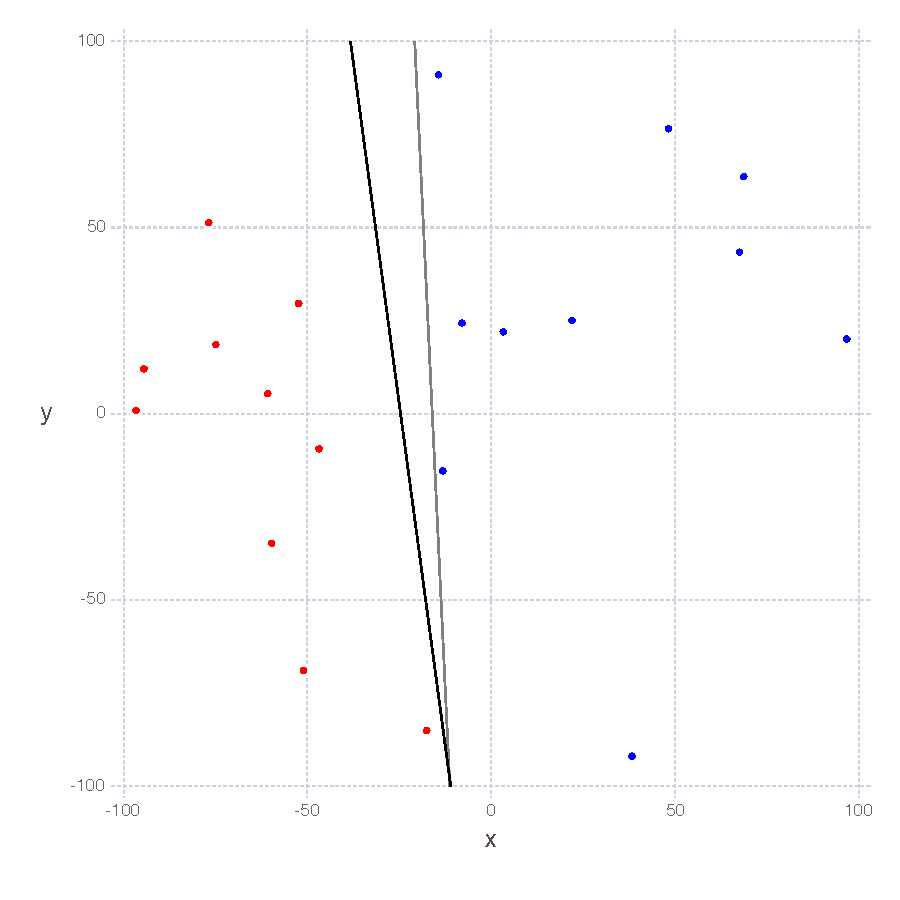
\includegraphics[width=\textwidth]{problem_1_4b.pdf}
	\caption{The solution for problem 1.4 b).  The algorithm took 1,608 iterations to find a valid hypothesis. The final hypothesis and the target function are not as good of a match as they could be.  This has to do with the implicit error measure that is used in the current perceptron algorithm; because we require that the data be linearly separable, our error measure is ``the first hypothesis that fits''.  This is a poor error measure because it is unrealistic, non-deterministic, and very loose.  It is unrealistic because noise in real datasets could lead to data sets with no match.  It is non-deterministic because there are an infinite number of equally good hypothesis (any hypothesis that fits is equally good), and the PLA will pick a hypothesis depending on the order that mis-miscategorized points are iterated over.  Finally, the hypotheses that are chosen are usually just barely correct and hug the current data.  For example, in this case the hypothesis mis-categorizes a large area unnecessarily.  This could be improved upon by using least-squares or some other error measure.}
\end{figure}

\begin{figure}
	\centering
    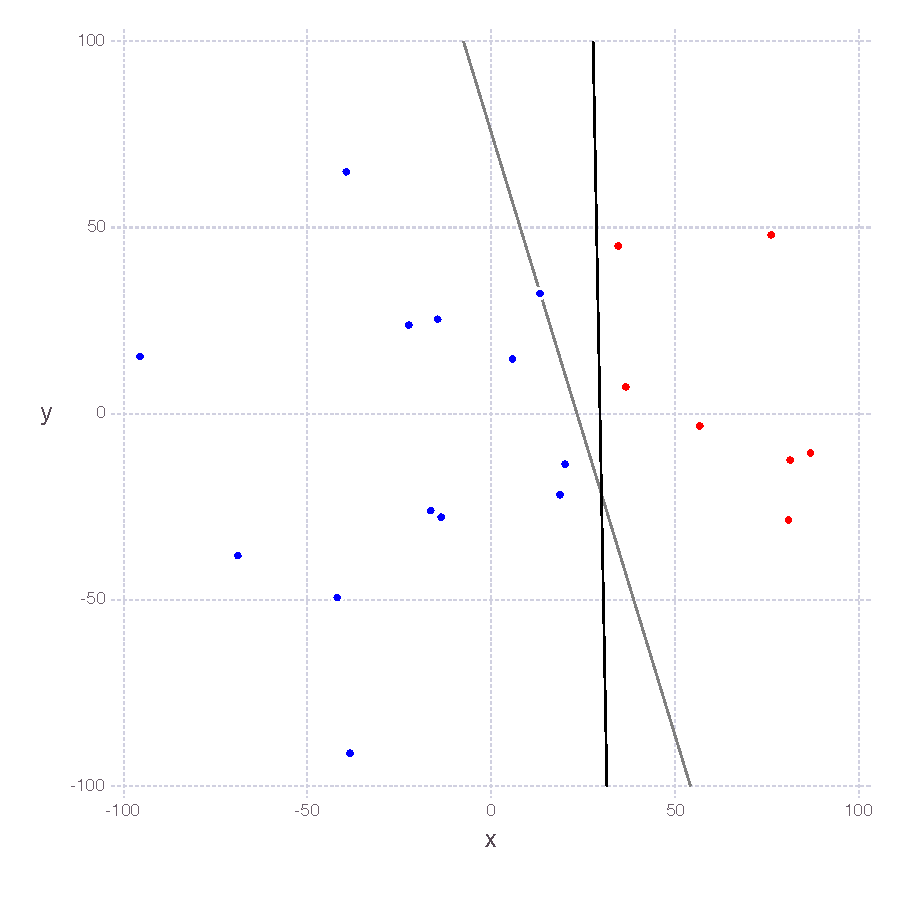
\includegraphics[width=\textwidth]{problem_1_4c.pdf}
	\caption{The solution for problem 1.4 c).  The algorithm took 184 iterations to find a valid hypothesis.}
\end{figure}


\begin{figure}
	\centering
    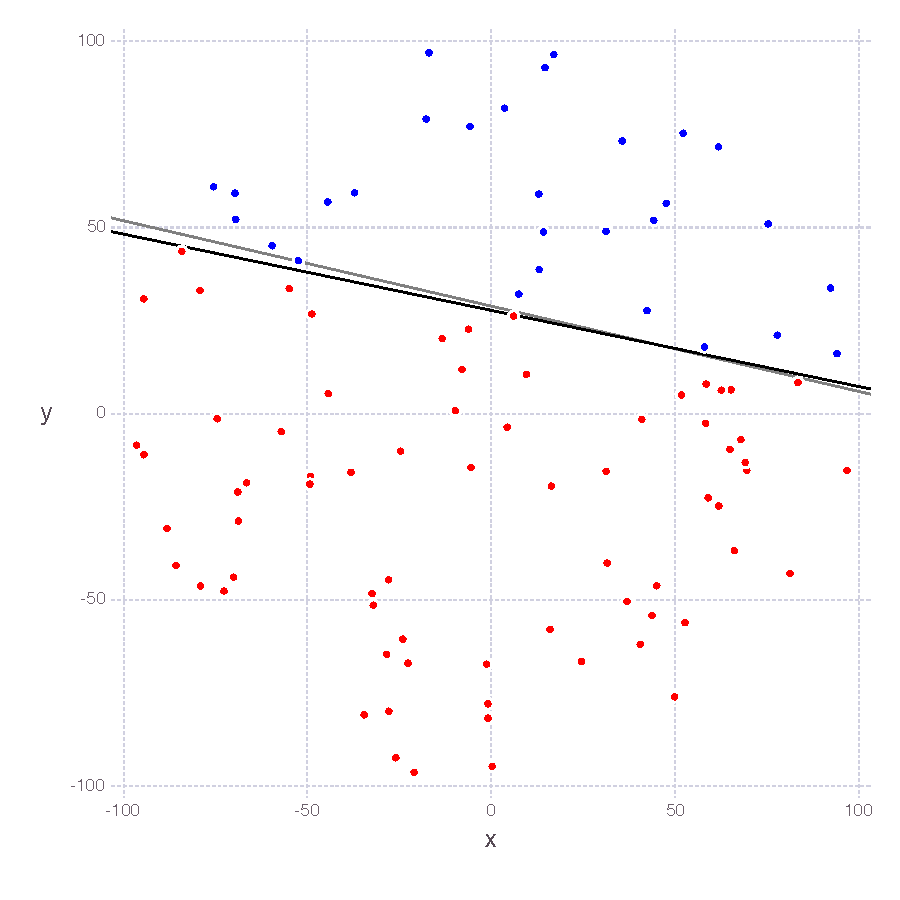
\includegraphics[width=\textwidth]{problem_1_4d.pdf}
	\caption{The solution for problem 1.4 d).  The algorithm took 34,803 iterations to find a valid hypothesis.}
\end{figure}


\begin{figure}
	\centering
    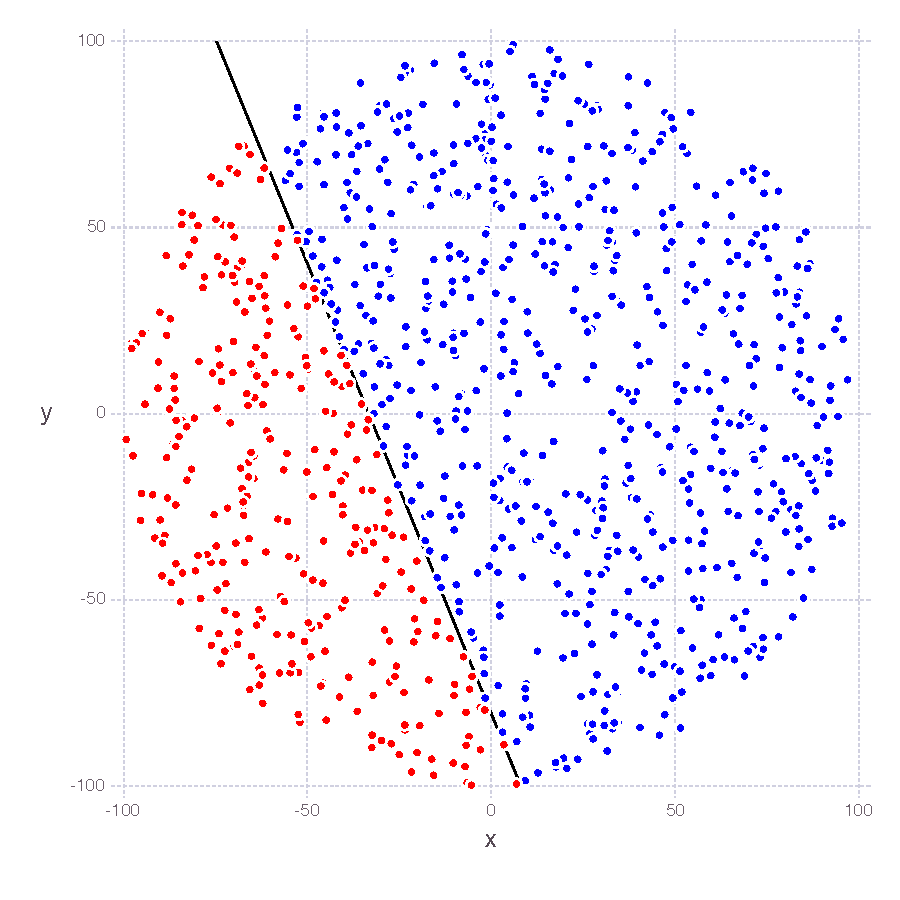
\includegraphics[width=\textwidth]{problem_1_4e.pdf}
	\caption{The solution for problem 1.4 e).  The algorithm took 1,359,257 iterations to find a valid hypothesis.  Note that the larger the data density the longer the algorithm takes to converge, but the more accurate the response is.}
\end{figure}


\begin{figure}
	\centering
    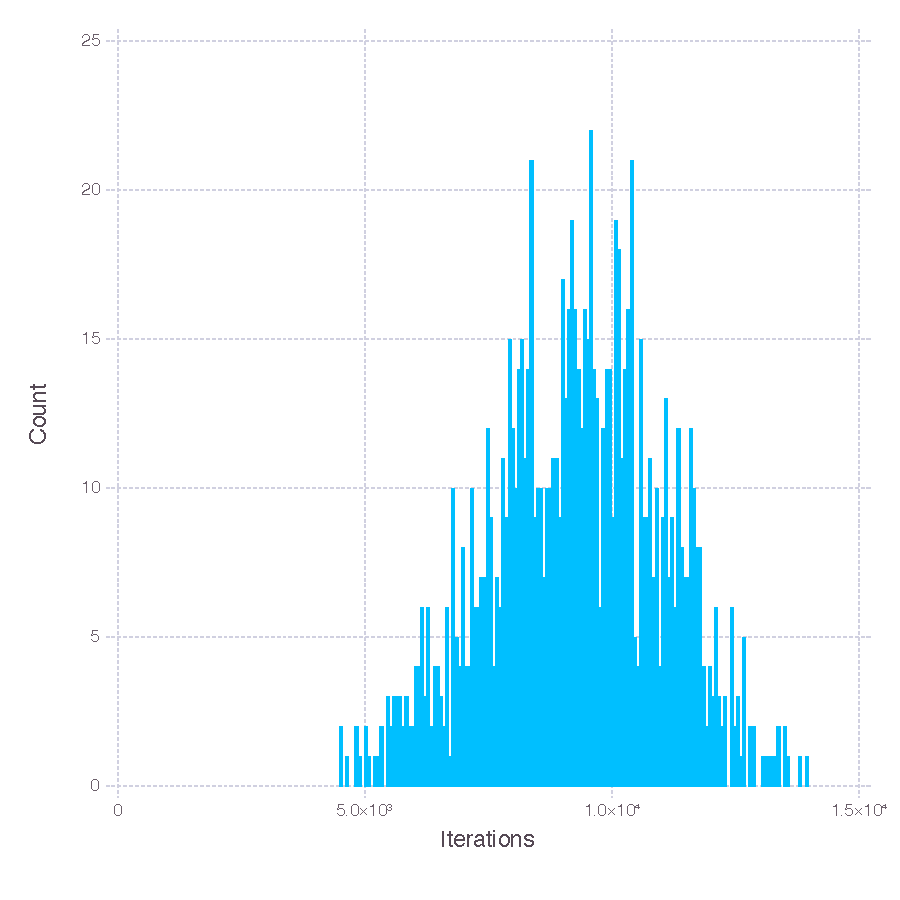
\includegraphics[width=\textwidth]{problem_1_4g.pdf}
	\caption{The solution for problem 1.4 f) and g).  }
\end{figure}


\begin{figure}
	\centering
    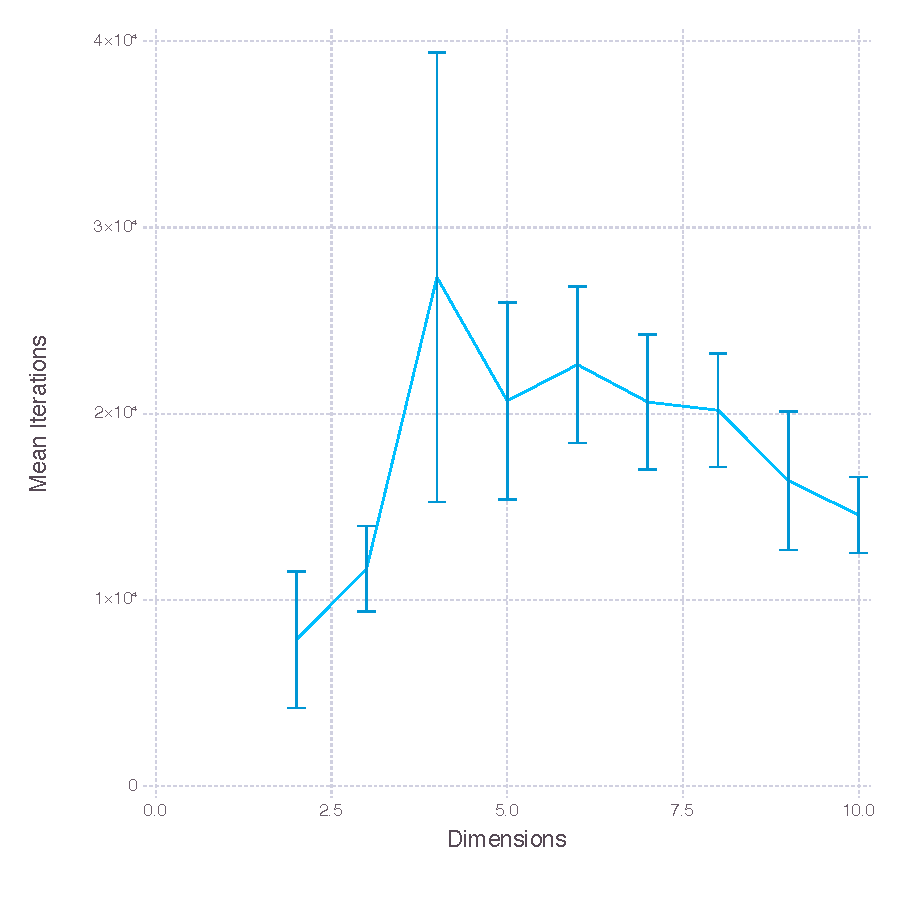
\includegraphics[width=\textwidth]{problem_1_4h.pdf}
	\caption{The runtime does not appear to increase as the dimensionality increases.  The runtime was averaged over 100 runs (using 100 data points) for each dimension.  Intuitively this makes sense, as each dimension is updated in parallel, furthermore there is nothing in the convergence bound proved in problem 1.3 that implies dimensionality would matter.  The variability appears to decrease as the number of dimensions increases.  This is likely because $R$ will increase as the number of dimensions increases, because most of the points will exist near the edges of the $n$-sphere.}
\end{figure}

Note that the choice of $f$ impacts the convergence speed a lot.  Thus if $f$ is being randomly chosen, the approach that it is generated could potentially alter some of the trends investigated in this problem.  For example, if you pick your plane by selecting a random point in your $n$-sphere and using its direction as the normal and its magnitude as the offset, then as $n$ increases the likelihood of the plane cutting through the edge of the $n$-sphere increases, and in the extreme case all of the points may be of a single type.  On the other hand, if $f$ is chosen to slice near the center of the $n$-sphere, then this won't be the case.


\section*{Problem 1.6}

a) $\p_\textrm{binomial}(\nu = 0 | N = 10, \mu) = \dbinom{10}{0} \mu^0 (1 - \mu)^{10 - 0} = (1 - \mu)^{10}$.
\\\\
b, c) The probability that at least one of M samples of 10 has $\nu = 0$ is equivalent to one less the probability of all of them not having $\nu = 0$.  Let $S_i = \p(\textrm{Sample $i$ has $\nu \ne 0$})$.
\begin{align*}
    1 - \prod_{i = 1}^{M} S_i = 1 - (1 - \p_\textrm{binomial}(\nu = 0 | N = 10, \mu))^M
\end{align*}
Here are the numerical values to five places:
\\\\
\begin{tabular}{|r|c|c|c|}
    \hline
    & $\mu = 0.05$ & $\mu = 0.5$ & $\mu = 0.8$ 
    \\ \hline
    (a) & 0.59874 & 0.00098 & 0.00000 
    \\ \hline
    (b) & 1.00000 & 0.62358 & 1.00010 
    \\ \hline
    (c) & 1.00000 & 1.00000 & 0.09733 
    \\ \hline
\end{tabular}

\section*{Problem 1.8}
a)
\begin{align*}
\p[t \ge \alpha] &= \int_\alpha^\infty p_t(T) dT \\
&\le \int_\alpha^\infty p_t(T) \frac{T}{\alpha} dT \\
&\le \int_\alpha^\infty p_t(T) \frac{T}{\alpha} dT + \int_0^\alpha p_t(T) \frac{T}{\alpha} dT \\
&= \e[t]/\alpha.
\end{align*}
Why not use $<$ for the first inequality?  Given that $T/\alpha \le 1$ within the integral, this may appear justified, however if $p_t(T) = \delta(T - 1)$ and $\alpha = \lim_{\epsilon \rightarrow 0} 1 - \epsilon$, then all of the probability density is centered where $T/\alpha = 1$; this case is why the first equality is less than \emph{or equal} to.
\\\\
b) The random variable $(u - \mu)^2$ is non-negative, and $\e[(u - \mu)^2] \equiv \sigma^2$, thus using (a) we have $\p[(u - \mu)^2 \ge \alpha] \le \frac{\sigma^2}{\alpha}$.
\\\\
c) The expected value operator is linear, thus $\e[u] = \frac{1}{N}\sum_{n=1}^N \e[u_n] = \mu$.  Given that the set of $u_n$ are iid, the variance is linear $\var[u] = \frac{1}{N^2}\sum_{n=1}^N \var[u_n] = \sigma^2/N$.  Using the same logic as in (b) we have the solution.  

\section*{Problem 1.9}

a) Similarly to the first part of the previous problem
\begin{align*}
\p[t \ge \alpha] &= \int_\alpha^\infty p_t(T) dT \\
&\le \int_\alpha^\infty p_t(T) e^{s(t - \alpha)} dT \\
&\le \int_\alpha^\infty p_t(T) e^{s(t - \alpha)} dT + \int_{-\infty}^\alpha p_t(T) e^{s(t - \alpha)} dT \\
&= e^{-s \alpha} \int_{-\infty}^\infty e^{st} p_t(T) dT \\
&= e^{-s \alpha} T(s).
\end{align*}
b) A basic property of moment generating functions (e.g. $T(s)$) is that the m.g.f. of a sum is the product of their m.g.f.s, hence we have $\e_u(\exp(su)) = \e_u(\exp(\frac{s}{N}(u_1 + u_2 + ... + u_N)) = U(\frac{s}{N})^N$, thus we have:
\begin{align*}
    \p[u \ge \alpha] &\le (e^{-s\alpha} U(s))^N.
\end{align*}
c) For a fair coin, we have $p(t) = \frac{1}{2}(\delta(t) + \delta(t - 1))$, hence $U(s) = \frac{1}{2}(1 + e^s)$. By inspection we see that $y(s) \equiv e^{-s\alpha}U(s)$ has no global maximum, and a single global minimum so long as $0 < \alpha < 1$, hence to minimize $y$ we take its derivative with respect to $s$, equate it to 0, and solve for $s_\textrm{min}$.
\begin{align*}
    \frac{d}{ds} y(s) &= \frac{1}{2}[(-\alpha)e^{-\alpha s} + (1 - \alpha)e^{s(1 - \alpha)}] \quad \Longrightarrow \\
    0 &= (-\alpha)e^{-\alpha s_\textrm{min}} + (1 - \alpha)e^{s_\textrm{min}(1 - \alpha)} \quad \Longrightarrow \\
    0 &= (-\alpha) + e^{s_\textrm{min}} - \alpha e^{s_\textrm{min}} \quad \Longrightarrow \\
    s_\textrm{min} &= \textrm{ln}\left(\frac{\alpha}{1 - \alpha}\right).
\end{align*}
Note we care about $s_\textrm{min}$ because it defines the upper bound for $\p[u_n \ge \alpha]$ ($s$ is a free parameter on the rhs of the inequality in part (b)), after substituting $s_\textrm{min}$ into $y(s)$ we have:
\begin{align*}
    \p[u_n \ge \alpha] &\le \frac{(1 - \alpha)^{\alpha - 1}}{2 \alpha^\alpha}.
\end{align*}
\\\\
d) Because $y(s) > 0$ for all $s$, the minimum of $y(s)^N$ occurs at the same location.  Hence using the results of (b) and (c) we have
\begin{align*}
    \p[u \ge \alpha] &\le \frac{(1 - \alpha)^{\alpha - 1}}{2 \alpha^\alpha}^N.
\end{align*}
This can be converted to the form in the textbook after a bunch of mathematical juggling that I don't have time to write out.

\section*{Problem 1.10}

a) 
\begin{align*}
    E_\textrm{off} &= 
    \begin{cases}
        \frac{1}{2}& \text{if $M$ is even},\\
        \frac{1}{2}\frac{M - 1}{M} & \text{if $M$ is odd and $N$ is even},\\
        \frac{1}{2}\frac{M + 1}{M} & \text{if $M$ is odd and $N$ is odd}.
    \end{cases}
\end{align*}
b) There are $2^M$ possible target functions that can generate $\mathcal{D}$.
\\\\
c) If $E_\textrm{off} = \frac{k}{M}$ then there are $k$ mismatches in the $M$ remaining $\vv{x}$, hence there are $\frac{M!}{k!(M - k)!}$ target functions $f$ that produce the specified off-training set error.
\\\\
d) The probability of having $E_\textrm{off} = \frac{k}{M}$ is the result of part (b) divided by the result of part (c), hence we have
\begin{align*}
    \e_f[E_\textrm{off}(h, f)] &= \sum_{k = 0}^{M} \frac{k}{M} \frac{M!}{k!(M - k)!} \frac{1}{2^M} \\
    &= \frac{1}{2^M} \sum_{k = 0}^{M} \frac{(M - 1)!}{(k - 1)!((M - 1) - (k - 1))!}  \\
    &= \frac{1}{2^M} \sum_{k = 0}^{M - 1} \frac{(M - 1)!}{k!((M - 1) - k)!}  \\
    &= \frac{1}{2}.
\end{align*}
e) Because we are only considering the off-training-set error, whether $A_1(\mathcal{D})$ generates $\mathcal{D}$ or not, the result from (d) should stand equally well for any hypothesis.

\section*{Problem 1.11}
\begin{align*}
    E_\textrm{in}(h, f) &= \frac{1}{N} \sum_{n = 1}^N e(h(\vv{x}_n), y_n))
\end{align*}
where $e$ is defined according to the risk matrices.  For example, the CIA pointwise error measure would be
\begin{align*}
    e(h(\vv{x}_n), y_n) &=
    \begin{cases}
        1000& \textrm{if $h(\vv{x}_n) = 1$ and $y_n = -1$},\\
        1& \textrm{if $h(\vv{x}_n) = -1$ and $y_n = 1$},\\
        0& \textrm{otherwise}.
    \end{cases}
\end{align*}


\section*{Problem 1.12}
a) We minimize $E_\textrm{in}$ by taking its derivative with respect to $h$ and solving for $h_\textrm{min}$ such that the result is 0.  Note we are assuming there is no global maximum.
\begin{align*}
    \frac{d E_\textrm{in}(h)}{dh} &= 2 \sum_{n = 1}^N (h - y_n)
     = 2 h N - 2 \sum_{n = 1}^N y_n \quad \Longrightarrow \\
     h_\textrm{min} &= \frac{1}{N} \sum_{n = 1}^N y_n.
\end{align*}
b) The method used in (a) doesn't work quite as well, because the derivative of the absolute value has a discontinuity.  However, within the scope of this problem, it makes sense to define the derivative of this discontinuity to be 0.  Hence we have
\begin{align*}
    \frac{d E_\textrm{in}(h)}{dh} &= \sum_{n = 1, h != y_n}^N \frac{h - y_n}{|h - y_n|}.
\end{align*}
The summand is either 1 or -1, hence the value that minimizes the summation must be a value of $h$ such that half the data points are at most $h$, and the other half are at least $h$---in other words, $h$ is the median.
\\\\
c) $h_\textrm{median}$ will be unaffected (unless perhaps you have a very small dataset), while $h_\textrm{mean}$ will diverge.

\end{document}

